\section{Projektkontext}
\subsection{Unser Team}
Unser Projektteams setzt sich aus einer interdisziplinären Gruppe von Studenten den Universität Bamberg zusammen.

\begin{itemize}
	\item \textbf{Anna Babicheva:} Angewandte Informatik.
	\item \textbf{Hannes Weber:} Angewandte Informatik.
	\item \textbf{Benedikt Freiburg:} Computational Social Science.
	\item \textbf{Peter Geiger:} Computational Social Science.
\end{itemize}

Aufgrund der unterschiedlichen Studienrichtungen bringt jedes Projektmitglied individuelle Perspektiven und Skillsets mit. Da Anna bereits Erfahrungen mit Wireframes hatte und sich gut auskannte, übernahm sie die Erstellung der App-Wireframes. Sie war ausserdem massgeblich an der konzeptionellen Ausarbeitung der Personas und des Designs beteiligt und wirkte ebenso an dessen praktischen Umsetzung mit. Hannes war für die grundlegenden Designaufgaben verantwortlich und legte damit das Fundament für die spätere Verfeinerung durch Benedikt und Peter. Als technisch versiertestes Mitglied übernahm er zudem die Entwicklung technischer Lösungen für diverse Designprobleme. Benedikt und Peter kümmerten sich um die Detailarbeit, erstellten Screens und setzten Feedback um.

Für Qualitätssicherung und Barrierefreiheit waren alle Mitglieder gemeinsam zuständig. Eine übergeordnete Projektleitung gab es nicht – wir arbeiteten in einer flachen, hierarchiefreien Struktur. Das verkürzte Kommunikationswege und erleichterte den Feedbackprozess.

\newpage

\subsection{Projektumfang}
\textbf{Unsere Kernfeatures belaufen sich auf:}
\begin{itemize}
	\item Blutdruck-, Puls- und EKG-Messungen sowie deren Interpretation.
	\item Kontaktfunktion für Angehörige / Notrufoption.
	\item Individuell einstellbare Medikamentenerinnerungen.
	\item Datenexport für Ärzte und Angehörige mit markanten Messwerten, Kontextkommentaren und Verlaufsdarstellung.
	\item Medi-KI-Chat, um schnelle Informationen mittels eines Chatbots zu erhalten und bei einfachen Fragen Ärztinnen und Ärzte zu entlasten.
	\item Möglichkeit für Angehörige, die Werte von Verwandten einzusehen.
	\item Korrespondierende UI für die App auf der Smartwatch.
\end{itemize}

\textbf{Die sich aus diesen Kernfeatures ableitenden Funktionen sind:}
\begin{itemize}
	\item Intuitiver Anmeldescreen.
	\item Datenschutzeinstellungen zur Einhaltung der GDPR.
	\item Verschiedene Abstufungen für Mitteilungen und Benachrichtigungen.
	\item Automatische Messungen zum Erkennen von Mustern im Krankheitsbild.
	\item Erstellung eines Symptomtagebuchs.
	\item Intuitive Sprachauswahl.
\end{itemize}

\begin{figure}[h!]
	\centering
	\begin{minipage}{0.3\linewidth}
		\centering
		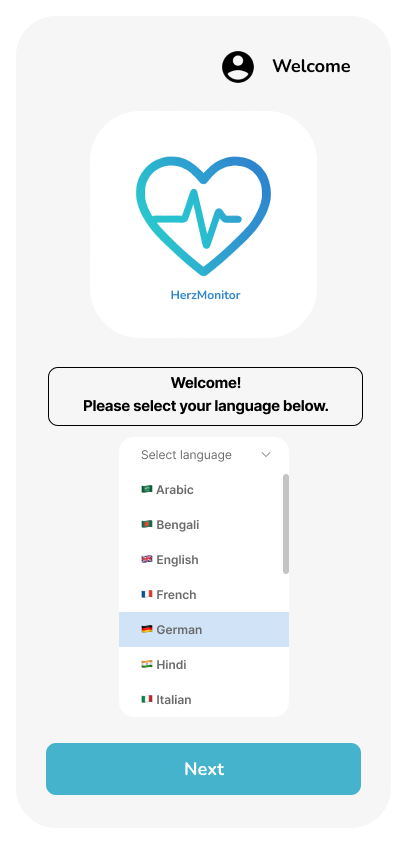
\includegraphics[width=\linewidth]{images/Sprachauswahl}
		\caption{Onboarding: Sprachauswahl}
		\label{fig:sprachauswahl}
	\end{minipage}
	\hfill
	\begin{minipage}{0.3\linewidth}
		\centering
		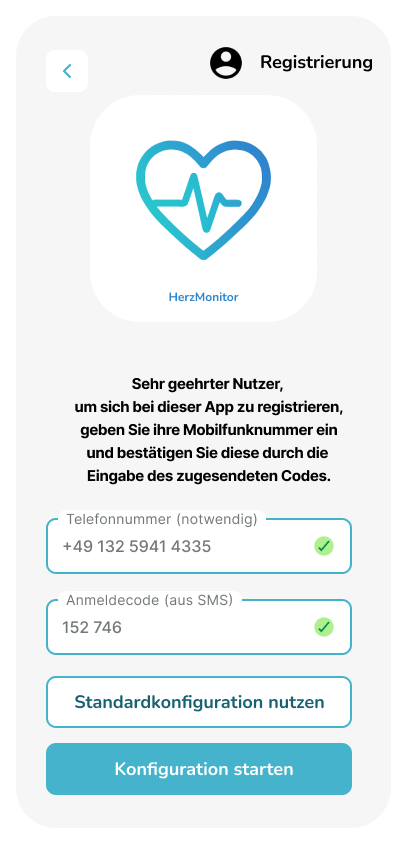
\includegraphics[width=\linewidth]{images/Registrierung}
		\caption{Onboarding: Registrierung}
		\label{fig:registrierung}
\end{minipage}
	\hfill
	\begin{minipage}{0.3\linewidth}
		\centering
		\includegraphics[width=\linewidth]{"images/Homescreen mit Symptomtagebuch"}
		\caption{Hauptmenü mit allen Features}
		\label{fig:homescreen-mit-symptomtagebuch}
	\end{minipage}
\end{figure}

\vspace{1em}

\subsection{Rahmenbedingungen}
\begin{itemize}
	\item Offenbacher Produktsprache: Grosse, selbsterklärende Buttons, klare visuelle Rückmeldungen, intuitive Navigationslogik, beruhigender Sprachstil.
	\item Sicherheit: Eindeutige Visualisierung von Schutzmechanismen (z.B. Schloss-Icon).
	\item Barrierefreiheit: Klare Kontraste, ausreichend grosse Bedienelemente, einfache Sprache. Möglichkeit, zusätzliche bzw. weiterführende Informationen anzuzeigen, falls dies gewünscht ist.
	\item Styleguide: Farbschema dominiert von Blau (Sicherheit), ergänzt durch Weiss, Hellgrau und sanfte Blautöne. Dieses Farbschema wird nur selten durchbrochen, um z.B. Warnungen wie „Auffälligkeit erkannt“ (\texttt{\#FF8000}, Orange) deutlich darzustellen.
\end{itemize}

\vspace{1em}

\begin{figure}[h!]
	\centering
	\begin{minipage}{0.3\linewidth}
		\centering
		\includegraphics[width=\linewidth]{images/Anzeige-Groß}
		\caption{Angezeigtes Icon wenn die Messung keine Auffälligkeiten aufweist.}
		\label{fig:anzeige-gros}
	\end{minipage}
	\hfill
	\begin{minipage}{0.35\linewidth}
		\centering
		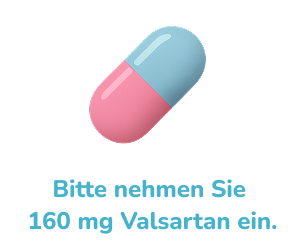
\includegraphics[width=\linewidth]{images/Einnahme}
		\caption{UI-Elemtente für die Medikamentenerinnerung}
		\label{fig:einnahme}
	\end{minipage}
\end{figure}
